\documentclass[times, utf8, seminar]{fit}

\usepackage{listings}
\usepackage{longtable}
\usepackage{xcolor}
\usepackage{float}
\usepackage{enumitem}
\usepackage{hyperref}
\usepackage{enumerate}
\usepackage{graphicx}
\usepackage{etoolbox}
\usepackage{datetime}
\usepackage{needspace}
\usepackage{titlesec}

\begin{document}
\widowpenalty=300
\clubpenalty=300
\setlength{\parindent}{0pt}

\lstset{
  language=bash,
  backgroundcolor=\color{gray!25},
  basicstyle=\ttfamily \footnotesize,
  breaklines=true,
  prebreak=\raisebox{0ex}[0ex][0ex] {\ensuremath{\hookleftarrow}},
  columns=fullflexible,
  keywords={},
  mathescape=false
}

%\title{Agilni \emph{software development}\newline \emph{Command-line} interfejs (CLI)}
\title{Agilni \emph{software development}\newline \emph{Toolbox} nove generacije developera}

% http://en.wikipedia.org/wiki/System_console
% http://en.wikipedia.org/wiki/Computer_terminal


% A terminal emulator, terminal application, term, or tty for short, is a program that emulates a video terminal within some other display architecture. Though typically synonymous with a command line shell or text terminal, the term terminal covers all remote terminals, including graphical interfaces. A terminal emulator inside a graphical user interface is often called a terminal window.


% programerski kalkulator


\author{Ernad Husremović}
\brindex{DL 2792}
\verzija {0.7.0}
\mentor{mr. Adil Joldić}

\maketitle

\tableofcontents

%\listoftables
%\listoffigures
\newpage

% abstract begin
%\begin{abstract}
%
%To be done 
%
%\keywords{open source software, OSS, Bosna i Hercegovina}
%\end{abstract}

% abstract end

\chapter{Uvod}

\emph{Human-computer interaction (HCI)}\footnote{Interakcija čovjek-računar} pročava zakonitosti interakcije čovjeka i računara.

Koncept grafičkog interfejsa (GUI), miš (mouse), ekran osjetljiv na dodir (eng. touch screen) su dobro poznati rezultati izučavanja HCI-a.

\section{Kategorizacija korisnika računara}

Različite skupine korisnika imaju različite zahtjeve i potrebe u kontekstu HCI-a. 

Tako malo dijete prepoznaje slike, ali ne razumije slova. Starijim i slabovidnim osobama potrebno je obezbjediti krupniji prikaz slova i znakova općenito. \enb{"Touch screen"} je intuitivan ulazno-izlazni uređaj, čak i za dijete od tri-četiri godine. Tastatura to nije. Lahko je zaključiti da pripadnost određenoj \emph{socijalnoj skupini} određuje moguće načine interakcije sa računarom.

Sljedeća bitna kategorizacija korisnika određena je poslovima koje korisnik obavlja na računaru. 

U uputstvima za korištenje software-a se ovakva kategorizacija korisnika jednostavno naziva "ciljna grupa". Softverska rješenja su redovno složeni proizvodi, namjenjeni za \emph{više ciljnih grupa} odjednom. Tako ćemo u uputstvima često naći sljedeće:
\begin{itemize}
  \item pogodno za početnike ...
  \item Ova opcija je namjenjena isključivo naprednim korisnicima ...
  \item Pristup dozvoljen samo Administratoru sistema\footnote{Administrator sistema - stručna osoba zadužena za funkcionisanje IT sistema}
\end{itemize}

\section{Produktivnost korisnika}

Dobro softversko rješenje bez dvojbe treba sa stanovišta \emph{ciljnog korisnika} biti \emph{produktivan} alat. Svrha software-a je pomoći da se obavi brže i efikasnije nega li bi to bio slučaj bez njega.

Produktivnost pretpostavlja niz elemenata koje je potrebno zadovoljiti:
\begin{itemize}
  \item tačnost - \emph{software} treba obezbjediti korsniku tačne rezultate
  \item fleksibilnost - software treba predvidjeti sve bitne varijante korištenja sa stanovišta korisnika
  \item robusnost - u slučaju problema i grešaka, gubici i zastoji korisnika trebaju biti minimalni
\end{itemize}

\section{Potrebni period učenja software-a (eng. \emph{Sofware Learning Curve})}

Poduktivnost "ne leži" samo u implementaciji softverskog rješenja. Produktivnost se postiže dobrim poznavanjem software-a od strane korisnika. Time dolazimo do još jedne bitne karakteristike software-a: Potrebni period učenja - \emph{Learning curve}.\footnote{Doslovni prevod na bio bi bosanski "krivulja učenja"}

Cilj je svakako da taj period bude što manji. Ono što je veoma bitno, jeste postizanje napretka u početnom periodu učenja. Ukoliko korisnik ne stekne osjećaj postignuća u početnom periodu, postoji velika mogućnost da će odustati od ponuđenog, posebno ako su mu na raspolaganju alternativna rješenja.

\section{Navike korisnika}

Kada se korisnik osposobi za korištenje određenog softverskog rješenja, on prirodom stvari stiče navike. Prosječan korisnik mnoge stvari obavlja po \emph{inerciji}. Čak i kada drugi korisnici postižu bolje rezultate, čak i kada su troškovi prelaska na druga rješenja minimalni, prosječan korisnik nije sklon promjenama software-a na koji je navikao. Stoga je, posebno u poslovnim primjenama, odabir odgovarajućeg rješenja veoma bitan korak.

\section{Kategorizacije programera}

Fokusirajmo se sada na programere kao posebnu ciljnu grupu. Sa stanovišta primarnih zaduženja, u domenu izrade poslovnih softverskih rješenja, adekvatna sljedeća podjela:

\begin{itemize}
  \item aplikativni programer - zadužen za održavanje i realizaciju standarndih funkcija softverskog rješenja, usmjerenih ka krajnjem korsniku 
  \item programer baznih funkcija (\emph{"core libraries"}) - zadužen za niže nivoe arhitekture software-a
\end{itemize}

Aplikativni programer je tako zadužen za izradu novog izvještaja "Pregled dugovanja kupaca koji su prekoračili rok dospijeća obaveze",  dok je "core" programer zadužen za realizaciju opcije "Razmjene podataka između prodavnica i centralne lokacije".  

Možemo nastaviti u dubinu sa ovom podjelom po sljedećim karakteristikama. Prema nivou vještina i iskustva: 
\begin{itemize}
  \item početnik - junior programer
  \item iskusni - senior programer
\end{itemize}

Softverska rješenja su složeni sistemi. Pojedine komponente traže dodatnu ekspertizu - specijalizaciju programera:
\begin{itemize}
  \item database programer
  \item programer korisničkog interfejsa (UI)
  \item programer web rješenja
     \begin{itemize}
          \item back-end
          \item front-end
      \end{itemize}
\end{itemize}

Ako posmatramo softverski projekat i njegov životni ciklus u cjelini, pored razvoja imamo i operacije podrške i instalacije\footnote{Često su u sve ove operacije programeri u većoj ili manjoj mjeri uključeni. Može se reći da je to čak pravilo ununtar manjih razvojnih timova}: 
\begin{itemize}
   \item poslovi podrške
   \item poslovi sistemske administracije
   \item poslovi razvoja i dizajna
\end{itemize}

\section{Agilni software development}

Agilni pristup se bazira na multi-funkcionalnim. Članovi takvog tima su posljedično generalisti\citep[str. 19]{agilesamurai}:

\begin{quote}
\emph{Kada formirate vaš tim, trebate generaliste, osobe koje nemaju problem raditi široki spektar stvari. Za programere, to znači naći osobe koje su sposobne raditi sa kompletnim tehnološkim stekom projekta (ne samo front-end ili back-end). Za testere i analiste, to znači osobe koje su spremne obaviti kako uobičajena testiranja, tako i detaljne analize korisničkih zahtjeva.}
\end{quote}

\section{Programerska produktivnost}

U predhodnih 20 godina, problemu povećanja programerske produktivnosti se pokušalo postići na mnoge načine. Izdvojimo načine koji su posebno interesantni za ovo izlaganje:

\begin{itemize}
  \item Izrada visoko sofisticiranih CASE\footnote{\url{http://en.wikipedia.org/wiki/Computer-aided_software_engineering#Tools}} alata
  \item Integrirana razvojna okruženja (IDE)\footnote{\url{http://en.wikipedia.org/wiki/Integrated_development_environment}} 
\end{itemize}

\subsection{CASE alati}

CASE alati su bili posebno popularan koncept kraja 80-ih i 90-ih godina (do ekspanzije interneta). CASE alati su pred sebe postavili iznimno ambiciozan cilj: napraviti okruženje koje će automatizirati kompletan životni ciklus razvoja software-a. Pri tome, zamišljeno je da se sam razvoj aplikacije realizira na visokom stepenu apstrakcije. Da bi se to postiglo, dizajneri CASE alata su trebali obezbjediti "kostur" aplikacije koji bi aplikativni programeri koristili kao polaznu tačku. Međutim, na kraju se pokazalo da tom konceptu nedostaje \emph{fleksibilnost}. Koliko god dobar dobro dizajniran CASE alati nisu mogli obuhvatiti sve moguće scenarije razvoja aplikacija. U konačnici, CASE alat može pružiti visoki stepen produktivnosti u početku razvoja, ali se ta prednost brzo "istopi" u kasnijim fazama razvoja aplikacija. 

Može se reži da su CASE alati pokušali pokušali kompleksne, kreativne faze razvoja software-a što više prebaciti u same CASE proizvode. Eksperti - dizajneri CASE alata prave ''kostur'' (eng. application skeleton), dok programeri - korisnici CASE-a realiziraju po tom već ustavnovljenom šablonu programska rješenja za krajnjeg korisnika. Zamisao je da se time posao aplikativnog programera svodi na manje više rutinski, dosta jednostavan posao.

Međutim, rezultat su bila rješenja koja nisu mogla zadovoljiti potrebama korisnika. CASE alati se jednostavno nisu mogli obuhvatiti svu raznolikost zahtjeva i potreba korisnika u realnom okruženju.

Drugi bitan faktor neuspjeha CASE koncepta je internet era, odnosno potreba za www\footnote{\url{http://hr.wikipedia.org/wiki/World_Wide_Web}} rješenjima. CASE alati nisu bili platforma za razvoj web rješenja\footnote{Web standardi su bili u povoju. Arhitektura web rješenja je u početku bila nejasna, fagmentacija web browsera velika}.

\subsection{IDE alati}

IDE alati su, za razliku od CASE alata ipak našli svoje mjesto u standardnom developerskom setu alata. Tu međutim treba imati na umu na opcije koje su u početku smatrane ključnim, marginalizirane po sličnom principu kao u slučaju CASE-a alata. Dobar primjer je funkcija Vizuelnog dizajnera formi (eng. Visual Forms Designer). Prve generacije IDE alata su ovu funkciju stavljale na vrh liste funkcija. Pokazalo se međutim da funkcije vizuelnog dizajniranja, čim aplikacija dosegne određeni nivo kompleksnosti, zna postati neadekvatna. Kada se to desi, vizuelni mod se napušta, i programer (ponovo) piše forme direktno u kodu. Takođe, ''Visual Forms'' alati do sada nisu postigli veliku primjenu na području razvoja web aplikacija, što je konceptu ''vizuelnog programiranja'' dodatno umanjilo na bitnosti. 

IDE okruženja su zato fokus razvoja usmjerili na produktivnost programera unutar \emph{source code} editora. Ključne opcije postaju funkcije koje asistiraju programeru:
\begin{itemize}
  \item automatsko kompletiranje imena funkcija, varijabli, klasa\footnote{Microsoftova implementacija \url{http://en.wikipedia.org/wiki/IntelliSense}}
  \item sugestije i pomoć programeru prilikom pisanja izvornog koda 
     \begin{itemize}
        \item pomoć pri formatiranju k\^oda - \eng{autoindent}
        \item provjera sintakse - \emph{syntax checking}
      \end{itemize}
  \item integrirano debugiranje
\end{itemize}

\section{Programski jezici}

\subsection{Java kao univerzalni programski jezik}

''Java''\footnote{\url{http://en.wikipedia.org/wiki/Java_(programming_language)}} programski jezik su početkom 90-tih mnogi smatrali univerzalnim programskim jezikom. Na kraju, ta očekivanja se nisu ispunila. Posebno su se pokazali nedostatnim sljedeće osobine ''java''-e\footnote{Preciznije je reći: ''Osobine JVM platforme'' s obzirom da je ''java'' samo jedan od jezika koji se izvršavaju na JVM\footnote{\url{http://en.wikipedia.org/wiki/Java_virtual_machine}} platformi}: 
\begin{itemize}
  \item java na strani web klijenta (java web plugin sistem)
  \item kompleksnost java serverskog steka J2EE\footnote{\url{http://radio-weblogs.com/0135826/2004/03/17.html}} 
\end{itemize}

U posljednjim implementacijama J2EE\footnote{\url{http://en.wikipedia.org/wiki/Java_Platform,_Enterprise_Edition}} su napravljeni značajni pomaci. Međutim, veliki broj developera je prihvatio alternativne tehnologije i programske jezike.

\subsection{Dinamički programski jezici}

Ekspanzija zahtjeva za web i mobilnim rješenjima je rezultirala pravom ''invazijom'' programskih jezika. 

Nova generacija developera, posebno u domenu razvoja web aplikacija, usvaja dinamičke programske jezike\footnote{\url{http://en.wikipedia.org/wiki/Dynamic_programming_language}}. 
 
Jedan od ključnih faktora tog trenda je značajno skraćen \emph{Learning curve} u odnosu na konvencionalne platforme (J2EE, .NET).

\subsection{Javascript, \emph{''Lingua franca''} web-a}

Ekspanzija web-a je dovela do neslućene ekspanzije ``Javascript`` programskog jezika\footnote{\url{http://en.wikipedia.org/wiki/JavaScript}}. Primarno zamišljen kao programski jezik \emph{web browsera}, javascript se počinje primjenjivati i van browsera:
\begin{itemize}
  \item mobilni klijent - appcelerator titanium\footnote{\url{http://www.appcelerator.com/platform/titanium-sdk}}
  \item \emph{server-side} - node.js\footnote{\url{http://nodejs.org}}
  \item \emph{database stored procedure} - plv8\footnote{\url{http://code.google.com/p/plv8js/wiki/PLV8}}
\end{itemize}
 

\section{Efekat masovnog usvajanja programske platforme}

Nakon teze o ''java''-i kao univerzalnom programskom jeziku, pojavila se teza o ''javascript''-u kao de-facto univerzalnom jeziku web-a\footnote{\url{http://www.codinghorror.com/blog/2007/05/javascript-the-lingua-franca-of-the-web.html}}. Cilj ovog materijala nije dokazati ili osporiti ovu tezu.

Međutim, svakako je bitno uočiti snagu usvajanja određene platforme, odnosno programskog jezika od strane velike grupe korisnika. 

\emph{Web browser} i \emph{Internet} općenito su postali univerzalna računarska platforma. 

To je razlog što je nova generacija developera tako dobro usvojila javascript/HTML/CSS. To je razlog što mnogi programerski alati kao bazični koncept uzimaju familijarnost sa ovim tehnologijama\footnote{\url{http://wiki.developerforce.com/page/Native,_HTML5,_or_Hybrid:_Understanding_Your_Mobile_Application_Development_Options}}.

Usvajenje ovih tehnologija je doslovno natjerala tržišne lidere na strateške promjene:
\begin{itemize}
  \item ''Microsoft'' stavlja fokus na HTML5 pored sopstvene RIA\footnote{\url{http://en.wikipedia.org/wiki/Rich_Internet_application}} platforme ''Silverlight''\footnote{\href{http://www.technologyreview.com/view/426083/html5-triumphant-silverlight-flash-discontinuing}{\color{blue}{Trijumf HTML5 nad zatvorenim vendorskim tehnologijama}}}
  \item ''Adobe'' takođe fokus budućeg razvoja usmjerava na HTML5, pored Flash RIA platforme\footnote{\url{http://www.adobe.com/products/flash/flash-to-html5.html}}
\end{itemize}

Ako su se oni spremi ''odreći'' platformi koje su im obezbjeđivale dominaciju na tržištu, onda i svaki drugi učesnik u IT industriji treba, ako ništa drugo, dobro razmisliti o svojoj budućoj strategiji razvoja. 

\chapter{\emph{Toolbox} nove generacije developera}

Dinamički programski jezici (php, python, ruby, javascript) su generirali potrebe za razvojem nove generacije programerskih alata. 

Tu se pojavio značajan problem. Niz funkcija koje je relativno jednostavno implementirati kod \emph{strong-type}\footnote{\url{http://en.wikipedia.org/wiki/Strong_typing}} programskih jezika\footnote{Dobar je primjer \emph{autocomplete} funkcija IDE-a}, je teško realizovati kod dinamičkih jezika.

Nova generacija developera iz temelja mijenja svoj toolbox. Kako konvencionalni IDE alati manjkaju naprednom podrškom dinamičkim jezicima, oni ponovo istražuju alternativna rješenja.

\section{Povratak u prošlost - komandna linija i programerski editor}

Njihov odabir je krajnje interesantan. Oni u svakodnevnom radu intenzivno koriste ''starinske'' alate:
\begin{itemize}
  \item Umjesto IDE okruženja, koriste programerske editore\footnote{\url{http://net.tutsplus.com/tag/code-editors/}} vi, emacs\footnote{Oni konvencinalniji Notepad++, TextMate, jEdit}
  \item intenizvno koriste terminal i komandnu liniju\footnote{\url{http://en.wikipedia.org/wiki/Strong_typing}} 
\end{itemize}

\section{TDD umjesto \emph{debuggera}}

Podrške interaktivnom debugiranju dinamičkih jezika je, posebno u početku, bila na niskom nivou. Taj nedostatak je značajno uticao na pojavu nove paradigme programiranja: \emph{Test driven development} - (TDD)\footnote{\url{http://en.wikipedia.org/wiki/Test-driven_development}}.

TDD se brzo pokazao kao pozitivna programerska praksa koja utiče na povećanje kvaliteta izvornog k\^oda neovisno od nivoa podrške debugiranju. 

\section{Programerski editor umjesto IDE-a}

\subsection{\emph{Vi} editor} 

\emph{Vi} editor\footnote{\url{http://en.wikipedia.org/wiki/Vim_(text_editor)}} je svojom popularnošću kod nove generacije developera\footnote{\url{https://github.com/tpope}, \url{http://blog.sanctum.geek.nz/vim-koans/}} po mnogo čemu fenomen savremene istorije razvoja software-a.

\begin{figure}[H]
\centering
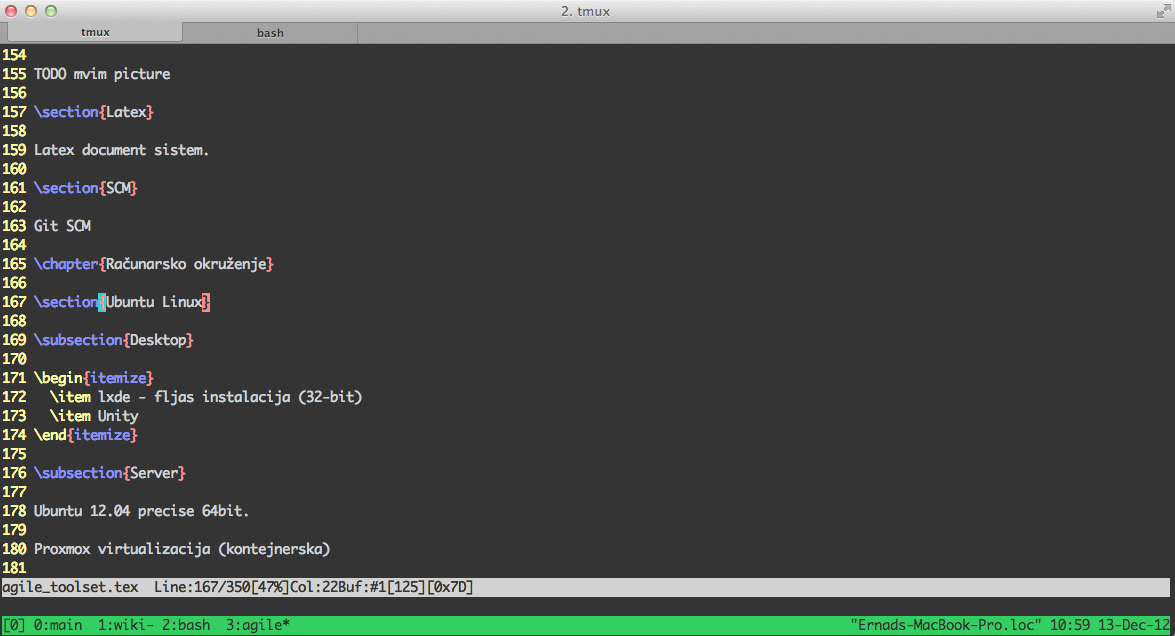
\includegraphics[width=14cm]{img/vim.png}
\caption{vim, terminal verzija}
\end{figure}

\begin{figure}[H]
\centering
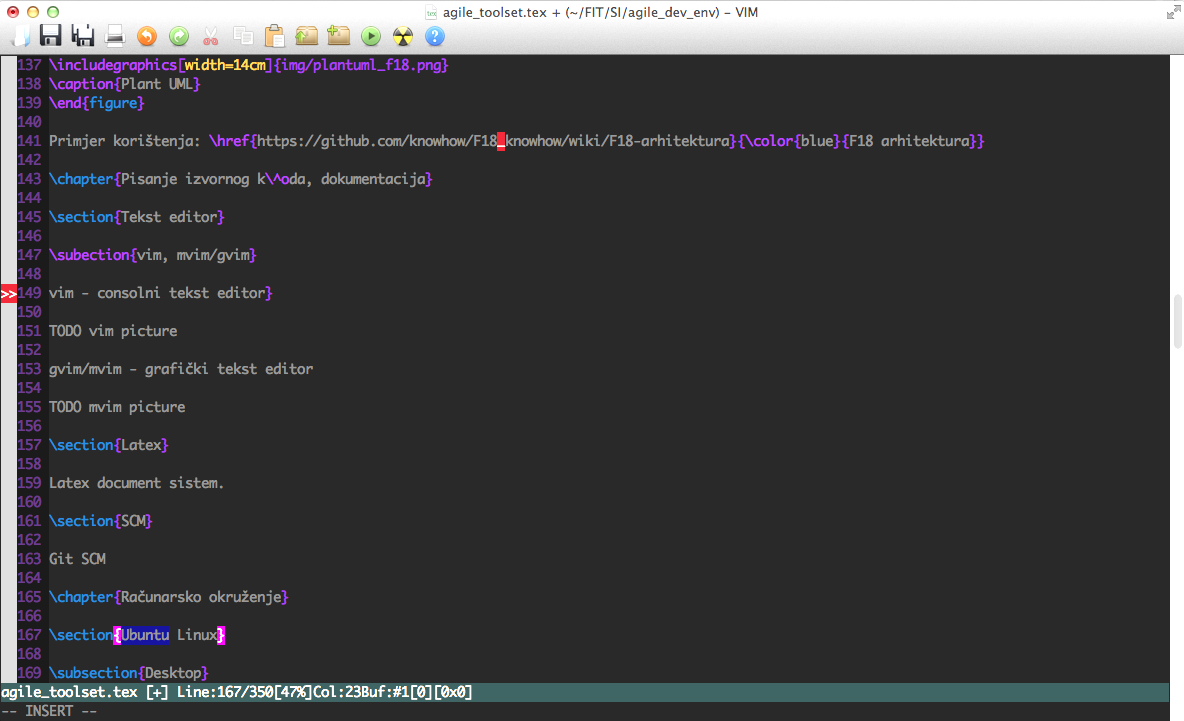
\includegraphics[width=14cm]{img/mvim.png}
\caption{mvim, Mac OS X grafička verzija vim editora}
\end{figure}

Vi editor je neintuitivan za početnika. \emph{''Learning curve''} ovog editora iznimno visok. \emph{vi} ima sasvim drugačiju paradigmu korištenja. Sa druge strane, \emph{vi} se uvijek nalazi na listi najpopularnijih programerskih editora\footnote{\href{http://tutorialzine.com/2012/07/battle-of-the-tools-which-is-the-best-code-editor}{\color{blue}{Pregled programerskih editora}}}.

\subsection{\emph{Vi} - editor koji ''misli'' kao programer}

\label{sec:vimaster}

Autor ovog teksta je često i sam isfrustriran \emph{vi}-om. Moji razlozi za usvajanje \emph{Vi} su bili sljedeći:
\begin{itemize}
 \item podrška linux serverima bez GUI interfejs-a
 \item Linux, Mac, Windows desktop - dostupnost GUI (gvim, mvim) ili terminal varijante, po izboru 
 \item najbolja podrška za \emph{harbour}\footnote{\footnote{http://en.wikipedia.org/wiki/Harbour_(software)}}
 \item brz rad i na računarima sa minimum RAM-a\footnote{Ovaj argument postaje sve manje bitan, ali i dalje postoje postojati uređaji koji imaju ograničene resurse - npr. \url{https://openwrt.org}}
\end{itemize}

Ukratko, \mvim{vi} je obavljao ono što trebam. Međutim, nikada nisam uspio do kraja usvojiti ''vi-način'' korištenja. Pripremajući se za ovaj rad nabavio sam knjigu ''Practical Vim, Edit Text at the Speed of Thought''\citep{pragvim}.

Čitajući knjigu brzo sam došao do sljedećeg zaključka:
\begin{itemize}
  \item Nakon 10-tak godina rada sa \emph{vi}-om, ja sam i dalje \emph{vi beginner} 
  \item Po svoj prilici, nikada neću ni postati \emph{vi master}\footnote{\url{http://blog.sanctum.geek.nz/vim-koans}}
\end{itemize}

Da bi se postalo \emph{vi masterom}, treba puno vježbe. Takođe, treba imati bistar um, um otvoren za usvajanje novih vještina. 

Učenje i istraživanje \emph{vi}-a će sigurno pomoći (posebno mlađem) programeru da podigne svoje vještine na viši nivo. To učenje će biti od koristi bez obzira da li će \emph{vi} biti primarni editor ili ne. \emph{Vi} ''tjera'' korisnika na \emph{rethink} svakodnevnih operacija pisanja programskog k\^oda. On pokazuje da uvijek postoji drugačiji i efikasniji način da se one obave. Mišljenja sam da je usvajanje tog \emph{rethink} pristupa ključni preduslov na putu ka \textbf{izvrsnosti} u programerskom poslu.

Bez obzira na ove zaključke, \emh{vi} ostaje moj izbor programerskog editora.  Koliko got puta se osjećao ''glupim'' pred ekranom \emph{vi}-a, ostaje zabavno otkrivati njegove mogućnosti i nove načine korištenja. Dodatno, pitanje razvojnog toolseta nije samo lično pitanje programera, nego pitanje od interesa za čitav razvojni tim. 
Ako ja i ne mogu postati \emph{vi master}, drugi članovi mogu. Svojim kolegama ipak mogu pomoći, posebno na početku, da bolje razumiju \emph{vi} i počnu razmišljati na ''vi-način''. Zato unutar svog razvojnog tima druge kolege potičem na korištenje \emph{vi}-a. Upravo to i jeste jedan od glavnih motiva za pisanje ovog rada.

\subsection{\emph{Vi} - primjer iz prakse}

Dugo sam razmišljao o tome šta bi to moglo pokazati snagu \emph{vi} koncepta, a da pri tome ne bude teško razumljivo čitaocu koji se po prvi put susreće sa \emph{vi}-om.

Onda sam se sjetio jednog primjera od prije par mjeseci. Zadatak je bio napraviti unos HTML ''select''-a za unos godine rođenja\footnote{Striktno gledajući, jedino dobro rješenje je napraviti dinammičko kreiranje takve kontrole kao što je to realizovano \href{https://github.com/hernad/FIT\_WT/blob/master/09\_2012/util.js\#L9}{\color{blue}{ovdje}}. S obzirom da tražimo najbrže rješenje, tu opciju isključujemo}

Otvorite vi editor i unesite sljedeći tekst\footnote{Ili kopirajte ovaj \href{https://gist.github.com/raw/4412263/1e751a7305ab75823689cfb7654304337f75336e/gistfile1.txt}{\color{blue}{gist}}}
\begin{lstlisting}[numbers=left]
<html>
<body>
Godina rodjenja:
<select name="datum_rodjenja">
   <option value="">Odaberi godinu</option>
   <option value="1910">1910</option>
</select>
</body>
</html>
\end{lstlisting}

Onda ukucajte sljedeće:

\begin{center}
\begin{tabular}{ l | l }
  \hline                        
   Kucati:    &  Opis \\ 
   \hline
   \verb+<ESC>+     & pređimo u ''Normal mode'' za svaki slučaj \\
   \verb+:set number<ENTER>+ &  prikažimo redne brojeve radi preglednosti \\
   \verb+6gg+    & skočimo na liniju 6 \\
   \hline
\end{tabular}
\end{center}

Nakon ovoga smo na poziciji drugog ''option'' elementa. Zastanimo malo. Razmislimo kao programer. Šta mi trebamo uraditi ? 
\begin{itemize}
  \item Trebamo iskopirati tekuću ''option'' liniju
  \item U toj novoj liniji trebamo povećati godinu na oba mjesta
  \item onda to trebamo ponoviti cca 100 puta
\end{itemize}

\subsection{\emph{Don't Repeat Yourself} (DRY) princip i \emph{vi}}
 
Vi ''macro'' sistem nam omogućava da gornje operacije realizujemo. Ali, kao programer - \textbf{bez ponavljanja}.

\begin{center}
\begin{tabular}{ |p{4cm}|p{10cm}| }
  \hline                        
   Kucati:    &  Opis \\ 
   \hline
   \verb+qa+     & započni snimanje \emph{vi} makroa u ''a'' registar \\
   \verb+0+      & idi na početak linije \\
   \verb+yy+     & snimi (''yank'') tekuću liniju u registar \\
   \verb+p+      & kreiraj (''paste'') novu liniju tako što ćeš je uzeti iz tekućeg registra (registar napunjenom predhodnom ''yank'' operacijom) \\
   \verb+<C-a>+  & <Ctrl> + 'a' - na tekućoj liniji pronađi broj i uvećaj ga za 1 (add operator, <C-x> je minus operator) \\
   \verb+w+      & otiđi na sljedeću riječ (pomjeri sa pozicije prvog broja) \\
   \verb+<C-a>+  & povećaj i drugi broj \\
   \verb+yy+     & ponovo snimi tekuću liniju u registar (da bi naredni paste uze posljednje uvećane brojeve) \\
   \verb+q+      & završi snimanje makroa.\\
   \hline
\end{tabular}
\end{center}

Stavimo sve na jedno mjesto. Dobijamo sekvencu: \verb+qa0yyp<C-a>w<c-A>yyq+. \newline Testirajmo naš makro sa \verb+@a+ (\emph{replay} makro ''a''). 

Trebali bi dobiti novu liniju \verb+<option value="1911">1911</option>+. 

Na kraju, zadajmo \emph{vi}-u da istu operaciju ponovi još 101 put. Ukucajmo: \verb+101@a+. 

Na kraju dobijamo konačni \href{https://gist.github.com/4412263}{\color{blue}{rezultat}}:

\begin{lstlisting}
<html>
<body>
Godina rodjenja:
<select name="datum_rodjenja">
   <option value="">Odaberi godinu</option>
   <option value="1910">1910</option>
   <option value="1911">1911</option>
      ....

   <option value="2012">2012</option>
</select>
</body>
</html>
\end{lstlisting}

\emph{Vi master} (vidi \ref{sec:vimaster}) ovakav zadatak doista može realizovati ''briznom misli''.

\subsection{Realizacija zadatka na drugi način: \emph{vi} + dinamički jezik}

Uzmimo dinamički jezik koji poznajemo. U njemu napravimo program koji će izgenerisati željeni tekst. Ruby program izgledao bi ovako:

\begin{figure}[H]
\begin{lstlisting}
#!/usr/bin/env ruby
puts "<select name=\"datum_rodjenja\">"

(1910..2012).each do |i|
       puts "   <option value=\"#{i}\">#{i}</option>"	
end

puts "</select>"
\end{lstlisting}
\caption{ruby generator teksta (\emph{/tmp/gen\_options.rb})}
\end{figure}

Sa \verb+r+ komandom učitavamo izlaz iz programa (ono što program pošalje na \verb+stdout+ uređaj) u tekući dokument\footnote{'':'' ukazuje na unos u komandom modu \emph{vi}-a.  Naravno, da bi ovo funkcionisalo \emph{ruby} interpreter postojati na sistemu}:

\begin{lstlisting}
:r !ruby /tmp/gen_option.rb
\end{lstlisting}

Uočavamo da je prva varijanta efikasnija kako sa stanovišta utroška vremena, kao i potrebne energije programera da dođe do cilja\footnote{Pod uslovom da je programer dobro uvježban i sa \emph{vi}-om i sa \emph{ruby}-jem (odnosno dinamičkim jezikom po izboru)}.

\subsection{IDE na \emph{Command-line} interfejsu}

U svjetlu ove teme interesantno je proučiti sljedeće pisane i video materijale:
\begin{itemize}
 \item  \href{http://blog.sanctum.geek.nz/series/unix-as-ide}{\color{blue}{Unix kao IDE}}
 \item \href{http://www.youtube.com/watch?v=za8FMIWYtUc}{\color{blue}{\emph{Remote} ''Pair programming'' sa ''tmux''-om}}\footnote{\url{http://tmux.sourceforge.net}, te knjiga ''tmux: Productive Mouse-Free Development''\citep{pragtmux}}
\end{itemize}

''Pair programming''\footnote{\url{http://en.wikipedia.org/wiki/Pair_programming}} je inače  jedna od ključnih developerskih praksi po XP metodologiji\citep{agileart}.

\section{Dolazeća generacija programerskih alata}

\emph{''Javascript everywhere''} princip širi se i na područje programerskih alata:
\begin{itemize}
   \item \emph{Adobe Brackets code editor} - \url{http://brackets.io}
   \item \emph{online} - alati u \emph{cloud}-u:
   \begin{itemize}
     \item \emph{CloudIDE} - \url{https://c9.io}
     \item \emph{Github code snippets} - \url{https://gist.github.com}
   \end{itemize}
\end{itemize}

Video nettuts+ ''A Peek At Brackets''\footnote{\url{http://www.youtube.com/watch?v=HZkrlX7jJcg}} ukazuje na inovativni pristup produktivnom pisanju Javascript/HTML/CSS k\^oda.

\begin{figure}[H]
\centering
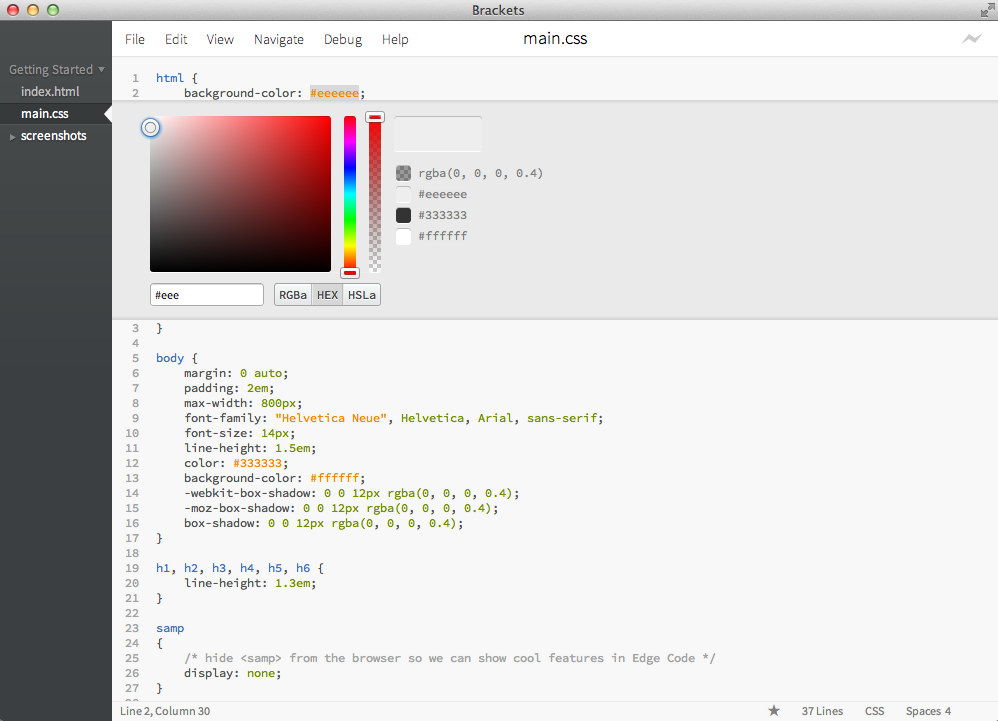
\includegraphics[width=12cm]{img/brackets_color_edit.png}
\caption{Brackets code editor - \emph{quick edit} ''color'' elementa}
\end{figure}

Programerski alati u \emph{cloud}-u je drugi značajan trend u ovoj oblasti. Socijalni aspekt \emph{online} alata - pojednostavljena komunikacija između developera su bitan katalizator ovih promjena.

\chapter{Komandna linija}

''Novi developer'' svakodnevno koristi terminal\footnote{\url{http://en.wikipedia.org/wiki/Terminal_emulator}} i komandnu liniju. U ovom poglavlju ćemo prikazati najbitnije načine korištenja \emph{command-line} alata.

\section{\emph{Command-line} interfejs (CLI) sa stanovišta HCI-a}
\label{sec:cli_hci}
Prednosti \emph{Command-line} interfejsa\footnote{\url{http://www.cs.man.ac.uk/~seanb/teaching/COMP10092/COMP10092-HCI.pdf}}:
\begin{itemize}
 \item brz i moćan za iskusne korisnike
 \item minimalna količina tipkanja (miš se ne koristi)
 \item može se koristiti u kombinaciji sa drugim korisničkim interfejsima
\end{itemize}

Nedostaci:
\begin{itemize}
\item izvršenje komandi sa malo ili bez pitanja korisnika
\item traži dobro poznavanje sistema i programa
\item bazira se na sjećanju - memorisanju komandi i sintakse
\item težak za učenje
\item sklon greškama
\end{itemize}

%Menu:
%
%Advantages
%Users don't have to memorize complex commands
%Structured navigation benefits novices and casual users
%Can shorten user learning time and effort
%Supports recognition memory
%
%
%Disadvantages
% May not be appropriate or efficient for some users and tasks
%Can force user through many levels of menus
%Users may get lost in menu hierarchies
%Menu terms and names may not be meaningful to users
%Use of modes forces users to follow the system's path
%
%

\section{\emph{Unix Pipe}}

\emph{Unix Pipeline}\footnote{\url{http://en.wikipedia.org/wiki/Pipeline_(Unix)}} je jednostavan, ali nadasve moćan koncept kreiranja složenih komandi preusmjeravanjem izlaza predhodne u ulaz naredne komande.

\begin{figure}[H]
\$ \verb+ps ax | grep MacVim | grep -v grep+
\begin{lstlisting}
  585   ??  S      1:13.89 /Applications/MacVim.app/Contents/MacOS/MacVim -psn_0_249917
86785   ??  Ss     0:00.23 /Applications/MacVim.app/Contents/MacOS/Vim -g -f --mmwaitforack
\end{lstlisting}

\caption{Pregled svih ''MacVim'' trenutno aktivnih procesa}
\end{figure}


\section{\emph{Read-eval-print-loop} (REPL)}

Dinamički jezik redovno sadrži REPL\footnote{\url{http://en.wikipedia.org/wiki/Read–eval–print_loop}} režim.
REPL omogućava interaktivni unos komandi dinamičkog programskog jezika.

\subsection{Programerski kalkulator bez limita - \emph{irb}}

Ruby\footnote{\url{http://www.ruby-lang.org}} REPL konzola naziva se \verb+irb+. 


\begin{figure}[H]
\$ \verb+irb+

\begin{lstlisting}
$ irb
irb> 228 % 15 # cjelobrojni ostatak
 => 3 
irb> 2**3 # stepenovanje
 => 8 
irb> a = 2**3 + 528/5.2
 => 109.53846153846153 
irb> b = Math.sin(0.2) + 2 * Math.cos(0.8)
 => 1.5920827494893923 
irb> a + 2.2 / b
 => 110.92029926059348
irb> # http://stackoverflow.com/questions/84421/converting-an-integer-to-a-hexadecimal-string-in-ruby
irb> "%x" % (0x0FF + 0x0EE) 
=> "1ed" 

\end{lstlisting}

\caption{ruby ''irb'' - kalkulator bez limita}
\end{figure}

\section{\emph{Regular expressions}}

\emph{Regular expressions}\footnote{\url{http://en.wikipedia.org/wiki/Regular_expression}} (regex) se koriste kod mnogih CLI alata. Takođe, moderni programski jezici imaju ugrađenu podršku za \emph{regexp}-e:
\begin{itemize}
   \item ruby podrška\footnote{\url{http://www.ruby-doc.org/core-1.9.3/Regexp.html}}
   \item grep \emph{text search} alat\footnote{\url{http://en.wikipedia.org/wiki/Grep}}
   \item sed \emph{stream editor}\footnote{\url{http://en.wikipedia.org/wiki/Sed}}
   \item awk\footnote{\url{http://en.wikipedia.org/wiki/AWK}}
   \item git grep (vidi \ref{sec:git})
   \item vim plugin ''CtrlP'' za brzu pretragu fajlova po imenu\footnote{\url{https://github.com/kien/ctrlp.vim}}
\end{itemize}

Poznavanje i korištenje \emph{regex}-a je bitan faktor produktivnosti programera.
 
% http://lifehacker.com/385929/best-text-editors

% http://sourceforge.net/apps/mediawiki/notepad-plus/index.php?title=Plugin_Central


% vim
% https://github.com/joonty/vdebug
% https://github.com/thoughtbot/vimulator


% http://en.wikipedia.org/wiki/Human_computer_interaction

% Human-omputer Interaction (HCI) involves the study, planning, and design of the interaction between people (users) and computers. It is often regarded as the intersection of computer science, behavioral sciences, design and several other fields of study. The term was popularized by Card, Moran, and Newell in their seminal 1983 book, "The Psychology of Human-Computer Interaction", although the authors first used the term in 1980[1], and the first known use was in 1975[2]. The term connotes that, unlike other tools with only limited uses (such as a hammer, useful for driving nails, but not much else), a computer has many affordances for use and this takes place in an open-ended dialog between the user and the computer.
% Because human–computer interaction studies a human and a machine in conjunction, it draws from supporting knowledge on both the machine and the human side. On the machine side, techniques in computer graphics, operating systems, programming languages, and development environments are relevant. On the human side, communication theory, graphic and industrial design disciplines, linguistics, social sciences, cognitive psychology, and human factors such as computer user satisfaction are relevant. Engineering and design methods are also relevant. Due to the multidisciplinary nature of HCI, people with different backgrounds contribute to its success. HCI is also sometimes referred to as man–machine interaction (MMI) or computer–human interaction (CHI).

% xmodmap i vim http://www.8t8.us/vim/vim.html

% tselect pattern http://stackoverflow.com/questions/4963019/search-for-a-tag

% unite-vim http://www.vim.org/scripts/script.php?script_id=3396

% https://github.com/hernad/neocomplcache

% http://en.wikipedia.org/wiki/Command-line_interface

%A command-line interface (CLI) is a means of interaction with a computer program where the user (or client) issues commands to a program in the form of successive lines of text (command lines).
%The command-line interface evolved from a form of dialog once conducted by humans over teleprinter machines, in which human operators remotely exchanged information, usually one line of text at a time. Early computer systems often used teleprinter machines as the means of interaction with a human operator. The computer became one end of the human-to-human teleprinter model. So instead of a human communicating with another human over a teleprinter, a human communicated with a computer.
%In time, the actual mechanical teleprinter was replaced by a glass tty (keyboard and screen, but emulating the teleprinter), and then by a terminal (where the computer software could address all of the screen, rather than only print successive lines).

%
%\section{Cloud i command line intefejs}

% http://www.h-online.com/open/news/item/Amazon-releases-preview-of-command-line-for-cloud-services-1774374.html

%
%
%\section{Zašto developer voli ''vim'', ''tmux'' i ''konzolu''}
%
%\section{Zašto se pojavio PowerShell ?}
%
%Jer su to ''Windows'' developeri tražli.
%
%Zašto su to tražili ?
%
%Radi automatizacije. GUI alati jesu lagani i intuitivni za rukovanje ali se te operacije ne mogu automatizirati.
%
%Koliko god konzola izgledala anahrona u odnosu na GUI interfejs, oni su uočili šta se na toj konzoli, sa bash i sličnim skriptnim jezicima može postići.
%

%\section{Zašto najnovija verzija titanium okruženja sadrži moćan CLI ?}
%
%Jer su to developeri tražili
%

\section{\emph{Command-line interface} (CLI) aplikacije}

CLI aplikacije se navode na komandnoj liniji - \emph(shell)-u operativnog sistema\footnote{Windows: cmd, PowerShell, Unix: sh, bash, zsh}.

\subsection{git klijent}
\label{sec:git}

Git je popularni SCM alat\footnote{Detaljnije u Git SCM \citep{agilegit}}

Postoji niz git klijenata sa GUI interfejsom\footnote{http://git-scm.com/downloads/guis}. 

\begin{figure}[H]
\centering
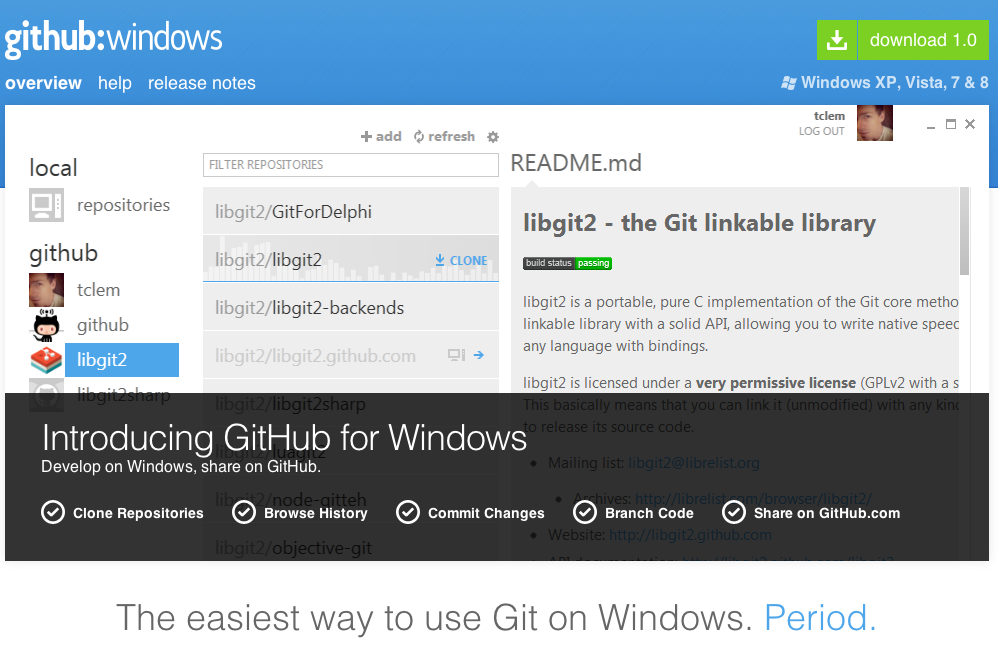
\includegraphics[width=12cm]{img/github_windows.png}
\caption{Naslovna stranica github GUI klijenta za Windows OS}
\end{figure}


Ipak, većina git korisnika koristi osnovnu, CLI verziju:

\begin{figure}[H]
\begin{lstlisting}
~$ git --help

=>

usage: git [--version] [--exec-path[=<path>]] [--html-path] [--man-path] [--info-path]
           [-p|--paginate|--no-pager] [--no-replace-objects] [--bare]
           [--git-dir=<path>] [--work-tree=<path>] [--namespace=<name>]
           [-c name=value] [--help]
           <command> [<args>]

The most commonly used git commands are:
   add        Add file contents to the index
   bisect     Find by binary search the change that introduced a bug
   branch     List, create, or delete branches
   checkout   Checkout a branch or paths to the working tree
   clone      Clone a repository into a new directory
   commit     Record changes to the repository
   diff       Show changes between commits, commit and working tree, etc
   fetch      Download objects and refs from another repository
   grep       Print lines matching a pattern
   init       Create an empty git repository or reinitialize an existing one
   log        Show commit logs
   merge      Join two or more development histories together
   mv         Move or rename a file, a directory, or a symlink
   pull       Fetch from and merge with another repository or a local branch
   push       Update remote refs along with associated objects
   rebase     Forward-port local commits to the updated upstream head
   reset      Reset current HEAD to the specified state
   rm         Remove files from the working tree and from the index
   show       Show various types of objects
   status     Show the working tree status
   tag        Create, list, delete or verify a tag object signed with GPG

See 'git help <command>' for more information on a specific command.
\end{lstlisting}
\caption{git CLI klijent}
\end{figure}

Zašto developeri napuštaju ''komfor'' GUI okruženja ? Zato što je CLI, kada se njime ovlada, efikasniji interfejs (vidi: \ref{sec:cli_hci}).

To je razlog zbog koga su se GUI alati uglavnom orjentisali na operacije najčešće korištene operacije, te operacije kod kojih je grafički prikaz evidentna prednost. U konkretnom slučaju, GUI klijenti su pogodniji za prikaz istorije promjena ili razlika između pojedinih verzija\footnote{Napomenimo da iskusni korisnici, ne preferiraju \emph{switch}-anje između GUI i CLI klijenta. Operacija \emph{switch}-anja sama po sebi narušava produktivnost.}


CLI klijent omogućava da se određene operacije obave na drugačiji način. Ako želimo pretražiti istoriju promjena, iskusni korisnik će prije posegnuti za \verb+git grep+ komandom, umjesto GUI prikaza istorije promjena:

\begin{lstlisting}  
NAME
       git-grep - Print lines matching a pattern

SYNOPSIS
       git grep [-a | --text] [-I] [-i | --ignore-case] [-w | --word-regexp]
                  [-v | --invert-match] [-h|-H] [--full-name]
                  [-E | --extended-regexp] [-G | --basic-regexp]
                  [-P | --perl-regexp]
                  [-F | --fixed-strings] [-n | --line-number]
                  [-l | --files-with-matches] [-L | --files-without-match]
                  [(-O | --open-files-in-pager) [<pager>]]
                  [-z | --null]
                  [-c | --count] [--all-match] [-q | --quiet]
                  [--max-depth <depth>]
                  [--color[=<when>] | --no-color]
                  [-A <post-context>] [-B <pre-context>] [-C <context>]
                  [-f <file>] [-e] <pattern>
                  [--and|--or|--not|(|)|-e <pattern>...]
                  [ [--exclude-standard] [--cached | --no-index | --untracked] | <tree>...]
                  [--] [<pathspec>...]
\end{lstlisting}


\chapter{Zaključak}


% -------------------------------------------------
\bibliography{literatura}
\bibliographystyle{fit}

\end{document}
